\section{Results and evaluation} \label{sc:results}
The algorithms were evaluated under the conditions presented in Section \ref{sc:experimental-validation}. The results of the evaluation for each algorithm are presented in the following sections.

\subsection{Specific evaluations}
Some of the considered algorithms require parameter configuration. Thus, the influence of the parameters as well as their importance for the process is presented in this section.

\subsubsection{Subspace}
The performance of the SDC as a function of the size of the image, as well as its capability in representing real SAR images, is investigated.

Since the proposed SDC is a global technique that operates directly on the whole image, it is essential to investigate its performance with the size of the image. This experiment is conducted by adding speckle noise to the synthetic image in Fig. \ref{fig:subspace-image1} at different noise levels and by calculating the PSNR gain from the despeckled image. 

The results obtained from the average values of 100 trials for the mix image in Fig. 4(a) are shown in Fig. 4(b). Here, the image size is varied from $500\times 500$ to $10 k\times 10 k$ pixels The results indicate better performance by the SDC with the growing size of the image. In general, the SDC performance improves by approximately $1.5$ dB when the size increases from $500\times 500$ to $1000\times 1000 $ and by $0.6$ dB when the size increases from $1000\times 1000 $ to $2000\times 2000 $. Similar results are obtained with portrait images, like Lena, Barbara, and boat. Generally speaking, the better performance of the SDC with the increased size of the image is mainly attributed to the improved structure of the estimated noise covariance matrix in terms of its diagonality. Close observation of the noise covariance matrix shows nonzero off-diagonal values when the size of the image is small and closer structure to diagonal as the image grows in size.

\begin{figure}[H]
	\centering
    \begin{tabular}{c c}
      \begin{varwidth}{0.5\linewidth}
        \subfigure{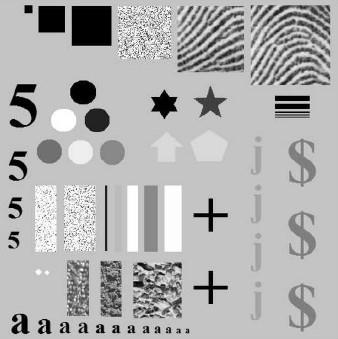
\includegraphics[width=20mm]{Figures/theory_subspace/a.jpg}}
      \end{varwidth}
      \begin{varwidth}{0.5\linewidth}
        \subfigure{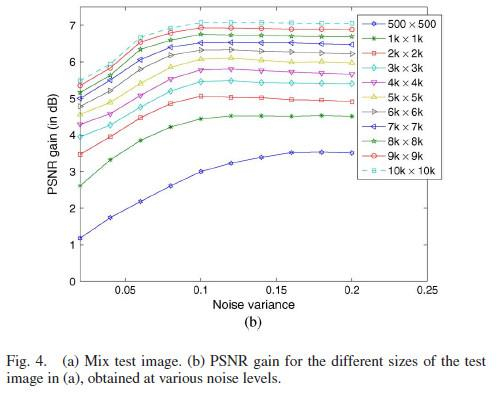
\includegraphics[width=20mm]{Figures/theory_subspace/2.jpg}}
      \end{varwidth}
  	\end{tabular}
  \caption{Synthetic image} 
  \label{fig:subspace-image1}
\end{figure}

To test the capability of the SDC in preserving SAR image details with r-dimensional principal subspace, the algorithm is run with the four images in Fig. \ref{fig:subspace-image2}(a), and the root-mean-square error (RMSE) metric is used to indicate its performance. In this experiment, the rank values are increased from 500 to around 8000 with a step size of 100, and the RMSE values are calculated and shown in Fig. \ref{fig:subspace-image2}. The results in Fig. \ref{fig:subspace-image2} clearly show the capability of the SDC in preserving the details of SAR images with a reduced-rank model. It is quite clear that the SDC can represent the four SAR images with an $RMSE < 0.1$ using rank values of $r \approx 4000$ for the mostly urban area.

\begin{figure}[H]
	\centering
    \begin{tabular}{c c}
      \begin{varwidth}{0.5\linewidth}
        \subfigure{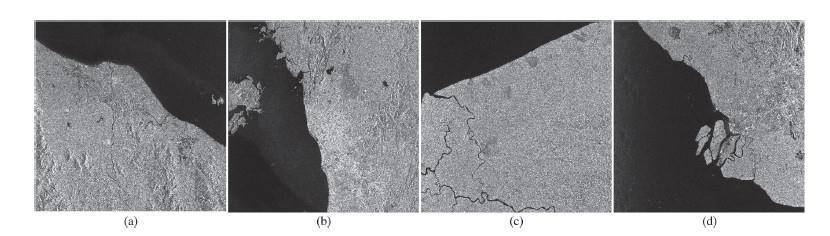
\includegraphics[width=20mm]{Figures/theory_subspace/image1.jpg}}
      \end{varwidth}
      \begin{varwidth}{0.5\linewidth}
        \subfigure{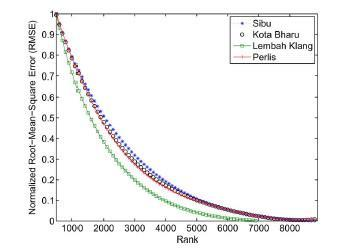
\includegraphics[width=20mm]{Figures/theory_subspace/image3.jpg}}
      \end{varwidth}
  	\end{tabular}
  \caption{Results of the SDC on SAR images} 
  \label{fig:subspace-image2}
\end{figure}

\subsubsection{K-SVD}
K-SVD algorithm, as presented in Section \ref{sc:description-ksvd}, requires to tune up some parameters. Each variable was varied during the evaluation process to observe its impact on the results. In general, the observed influence was the following:

\begin{itemize}
	\item Block size: The block size represents the dimension of the patch to consider. On one hand, when evaluating synthetic images, the higher the value of the parameter, the more blurred the result. On the other hand, the best results for SD-OCT was obtained when using a block size of 32 -- the biggest value tested for this parameter.
    \begin{figure}[H]
      \centering
     \begin{tabular}{c c c c c}
         \begin{varwidth}{0.5\linewidth}
           \subfigure{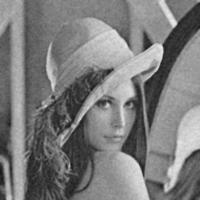
\includegraphics[width=16mm]{Figures/theory_ksvd/lena_block_size_4.jpg}}
         \end{varwidth}
         \begin{varwidth}{0.5\linewidth}
           \subfigure{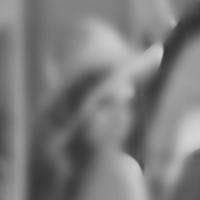
\includegraphics[width=16mm]{Figures/theory_ksvd/lena_block_size_32.jpg}}
         \end{varwidth}
     \end{tabular}
      \caption{Denoised images with K-SVD algorithm using different block sizes. On the left the block size is 4 while on the right is 32.} 
      \label{fig:influence-block-size}
    \end{figure}

	\item Dictionary size: This parameter determines the number of patches to consider for the dictionary. The size by itself does not modify the result dramatically.
    
    \begin{figure}[H]
      \centering
     \begin{tabular}{c c c c c}
         \begin{varwidth}{0.5\linewidth}
           \subfigure{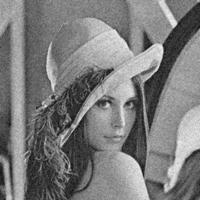
\includegraphics[width=16mm]{Figures/theory_ksvd/lena_dic_size_256.jpg}}
         \end{varwidth}
         \begin{varwidth}{0.5\linewidth}
           \subfigure{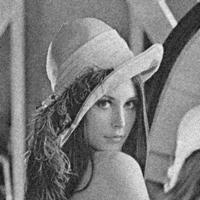
\includegraphics[width=16mm]{Figures/theory_ksvd/lena_dic_size_512.jpg}}
         \end{varwidth}
     \end{tabular}
      \caption{Denoised images with K-SVD algorithm using different dictionary sizes. On the left the dictionary size is 256 while on the right is 512.} 
      \label{fig:influence-dictionary-size}
    \end{figure}

	\item Trainnum: This parameter is related to the number of iterations performed during the training step. Usually, when it increases, the result is better. However, we observed that there is a limit for which no better result is obtained. It is required that its value must be greater or equal to the dictionary size.
   	\item Gain: The influence of this parameter is seen on the edges of the resulting images. When its value is decreased, the image is less denoised but the edges were better preserved.
   	\item Maxatoms: This parameter is related to the number of elements on the dictionary to consider when reconstructing a patch of the noisy image. The higher the value, the better the reconstruction but also the slower the algorithm gets. Thus, the idea is to find the minimum value such that the trade-off between reconstruction and computation time is balanced. 
    \item Noise: As stated previously, the level of distortion on the SD-OCT images is not known beforehand and this value is required by the K-SVD algorithm. Then, the estimation of this parameter is carried out. The method consists in taking an homogenous patch of the image and, by looking at the histogram, determine the sigma value. The observed value for sigma among the test set was around $10$. Moreover, we calculated this parameter for different retinopathy volumes getting similar results.
\end{itemize}

\subsubsection{PGPD} \label{sc:eva_pgpd}
After achieving result of PGPD denoising we tested our technique on the following parameters:
\begin{itemize}
\item the number of patches per group
\item patch search window. 
\end{itemize}
In the first experiment we vary the number of patches per group with initial value for number of patches being 10. Recall that PG is considering not the patches themselves, but patches minus mean of all the patches in the group. In the algorithm we find the correspondence between patch of our noisy image and the group of averaged patches. The results of algorithm performance are as follows:
\begin{figure}[H]
  \centering
  \begin{tabular}{c c c c}
      \begin{varwidth}{0.25\linewidth}
        \subfigure{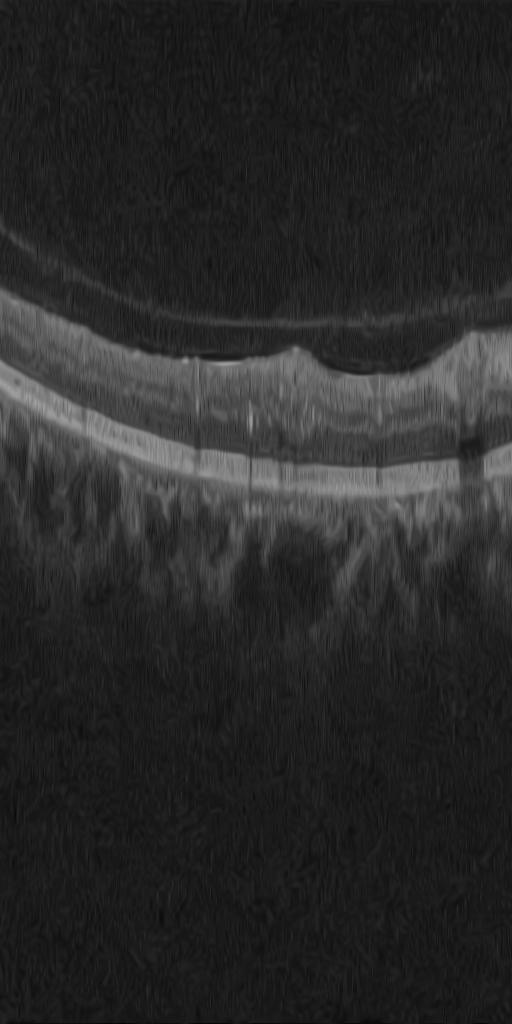
\includegraphics[width=20mm]{Figures/theory_PGPD/OCT7.jpg}}

      \end{varwidth}
      \begin{varwidth}{0.25\linewidth}
        \subfigure{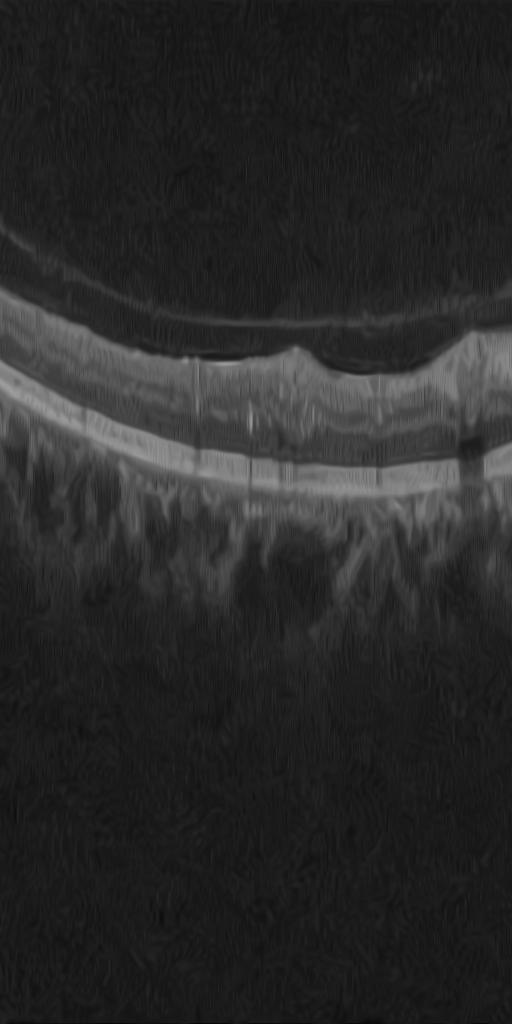
\includegraphics[width=20mm]{Figures/theory_PGPD/OCT11.jpg}}
      \end{varwidth}
      \begin{varwidth}{0.25\linewidth}
        \subfigure{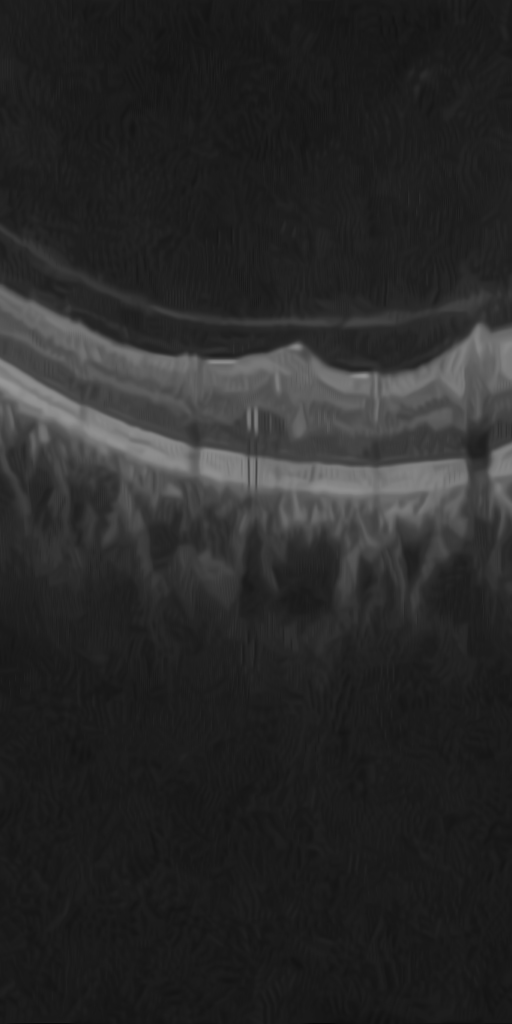
\includegraphics[width=20mm]{Figures/theory_PGPD/OCT20.jpg}}
      \end{varwidth}
      \begin{varwidth}{0.25\linewidth}
        \subfigure{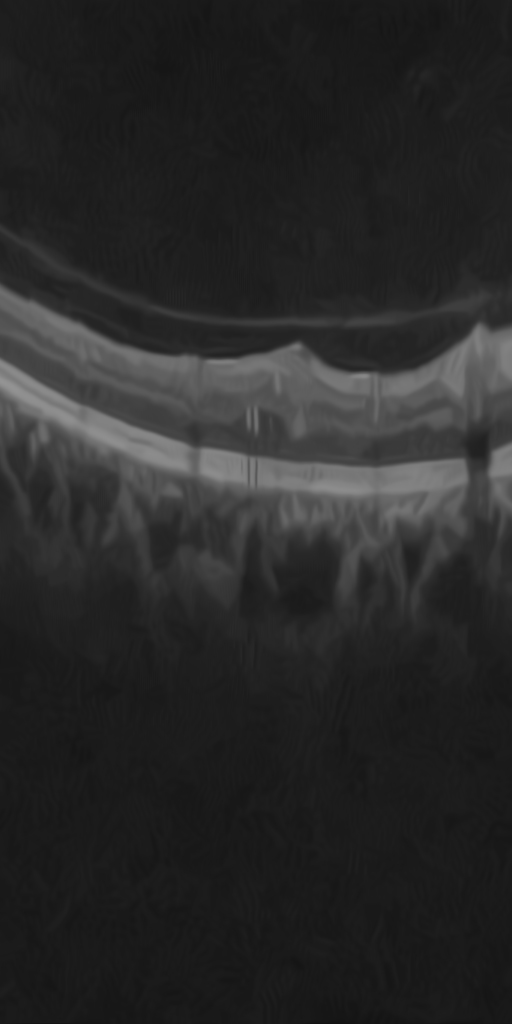
\includegraphics[width=20mm]{Figures/theory_PGPD/OCT40.jpg}}
      \end{varwidth}
  	\end{tabular}
  \caption{Retina denoising results with number of patches in group being from left to right :   7, 11, 20, 40.} 
  \label{fig:results_OCT}
\end{figure}
We can see that with value of patches per group being equal to 15, we reach saturation point where adding more images to group does not give any additional information,but instead makes the image blurry. We can look at this in the following way: when we increase the number of patches we reach the point when average of all patches is no longer similar to patches themselves which ruins data in PG and therefore match is no longer precise.Thus, we can draw a conclusion that the optimal number of patches per group should be the initial value selected -10.

In this section we are trying to estimate the affect of the PG search window on precision of patch mathing. PGPD algorithm searches for a patch of fixed size in the window $N\times N$ and we vary $N$. The results are as follows:
\begin{figure}[H]
  \centering
  \begin{tabular}{c c c}
      \begin{varwidth}{0.25\linewidth}
        \subfigure{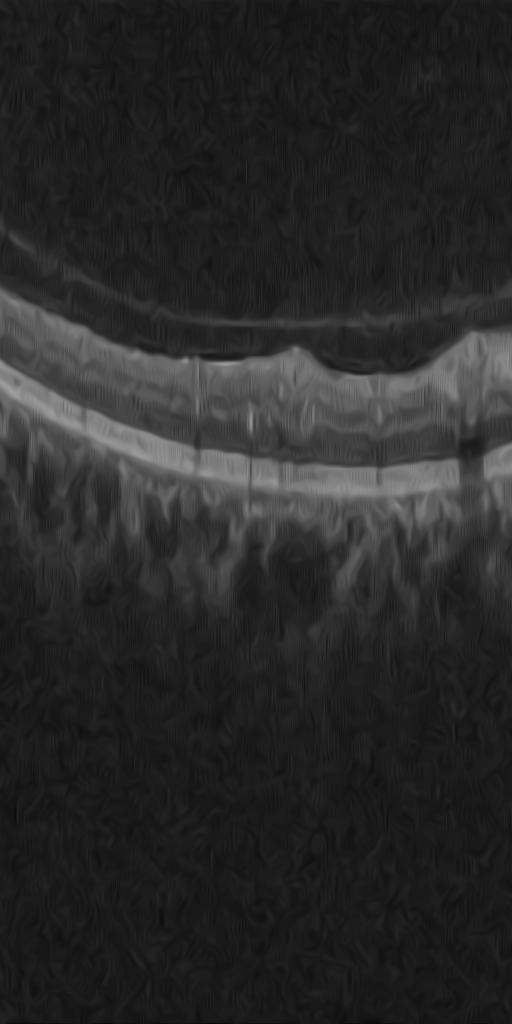
\includegraphics[width=20mm]{Figures/theory_PGPD/Win5.jpg}}

      \end{varwidth}
      \begin{varwidth}{0.25\linewidth}
        \subfigure{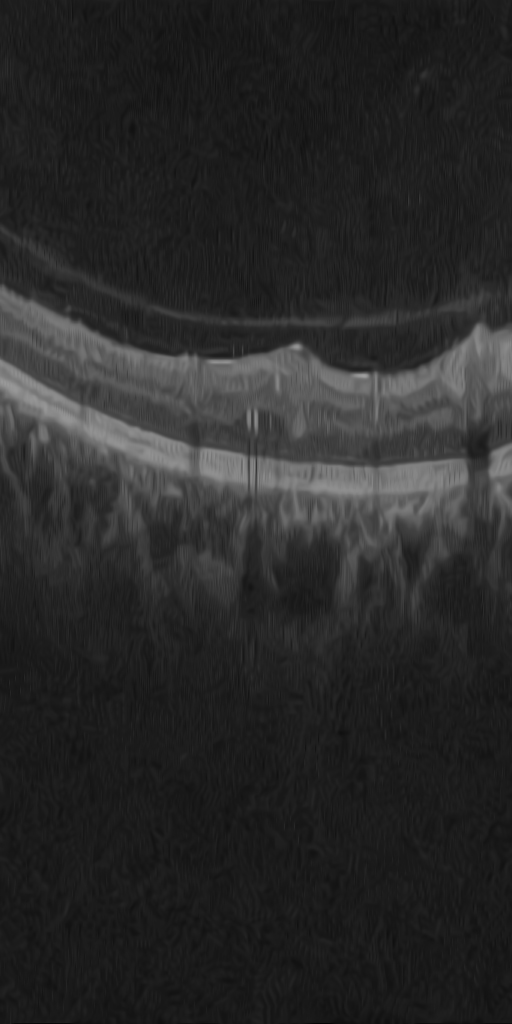
\includegraphics[width=20mm]{Figures/theory_PGPD/Win15.jpg}}
      \end{varwidth}
      \begin{varwidth}{0.25\linewidth}
        \subfigure{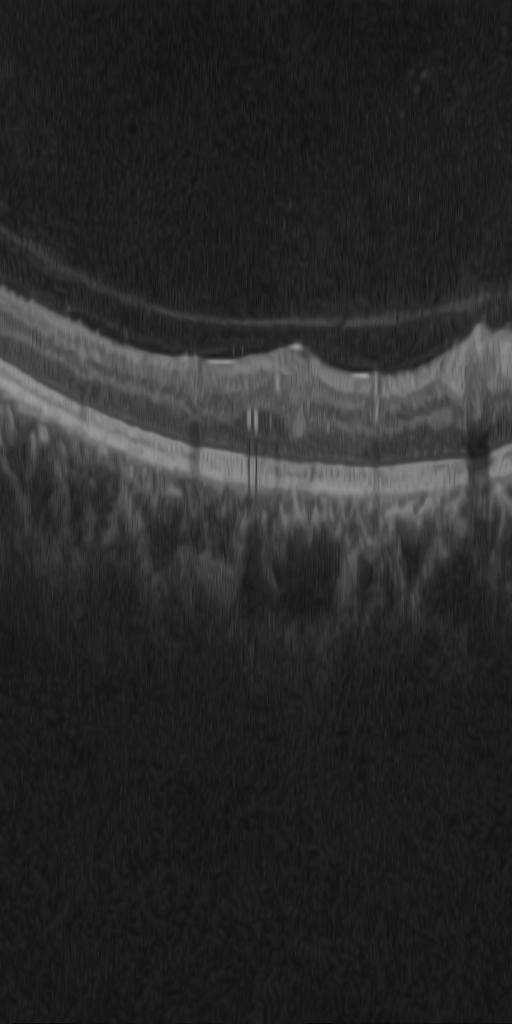
\includegraphics[width=20mm]{Figures/theory_PGPD/Win30.jpg}}
      \end{varwidth}
  	\end{tabular}
  \caption{Patch search window variation from left to right: $5\times5,15\times15,30\times30$ patches around initial patch.} 
  \label{fig:results_Win}
\end{figure}
In picture set we can observe that with increasing of the window size we get better results, but the drawback of such improvement is the computational time. We can observe that when reaching the parameter of N being 15, the further improvement of quality is miserable compared to needed computational time.

\subsubsection{NLM}
It is essential to determine the effect of various NLM filter parameters on denoised output. The three parameters that were tested with are filter size (f), search window (t) and degree of filtering (\(\sigma\)). The search window and filter size do not have any major visual effect on the output. As expected, increasing these parameters increases the execution time. However, \(\sigma\) used in the filter should be close to the original \(\sigma\) of the noise. Choosing very low values for \(\sigma\) parameter can lead to poor denoising, whereas choosing very high values would have the effect of image blurring. 

\subsection{Synthetic images} \label{sc:results_synthetic}

\subsubsection{Mean filter}
	Mean filtering is one of the simplest kernel-based smoothing techniques, which simply calculates the average value of pixels within its search window. However, this simplicity did not translate to good denoising results, underperforming most of the advanced methods. This is because it acts as a low-pass filter, discarding higher frequency components with no distinction between noise and signal. In addition, mean filtering affects the quality of the image by smoothing out edges, which degrades parts of the image without much noise. Given its extreme simplicity, the mean filter offers a good benchmark to compare with modern techniques.

\begin{figure}[H]
  \centering
  \begin{tabular}{c c c c c}
      \begin{varwidth}{0.5\linewidth}
        \subfigure{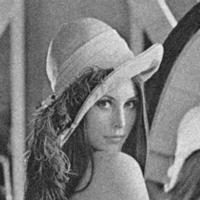
\includegraphics[width=16mm]{Figures/results_mean/lena_nor_f.jpg}}\\
        \subfigure{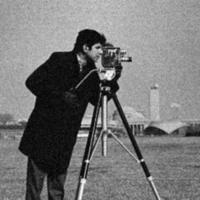
\includegraphics[width=16mm]{Figures/results_mean/cameraman_nor_f.jpg}}\\
        \subfigure{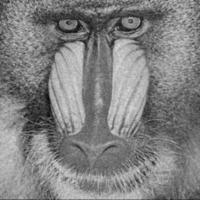
\includegraphics[width=16mm]{Figures/results_mean/baboon_nor_f.jpg}}
      \end{varwidth}
      \begin{varwidth}{0.5\linewidth}
        \subfigure{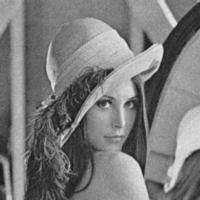
\includegraphics[width=16mm]{Figures/results_mean/lena_ric_f.jpg}}\\
        \subfigure{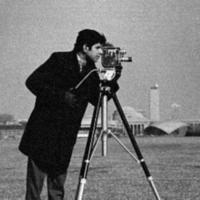
\includegraphics[width=16mm]{Figures/results_mean/cameraman_ric_f.jpg}}\\
        \subfigure{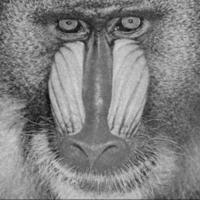
\includegraphics[width=16mm]{Figures/results_mean/baboon_ric_f.jpg}}
      \end{varwidth}
      \begin{varwidth}{0.5\linewidth}
        \subfigure{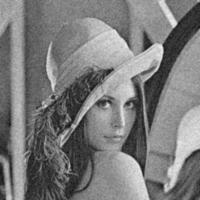
\includegraphics[width=16mm]{Figures/results_mean/lena_uni_f.jpg}}\\
        \subfigure{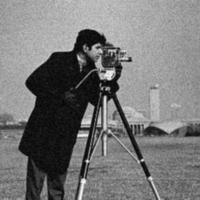
\includegraphics[width=16mm]{Figures/results_mean/cameraman_uni_f.jpg}}\\
        \subfigure{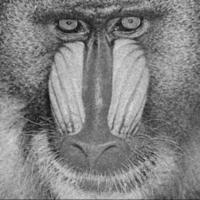
\includegraphics[width=16mm]{Figures/results_mean/baboon_uni_f.jpg}}
      \end{varwidth}
      \begin{varwidth}{0.5\linewidth}
        \subfigure{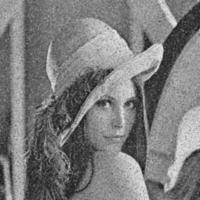
\includegraphics[width=16mm]{Figures/results_mean/lena_sp_f.jpg}}\\
        \subfigure{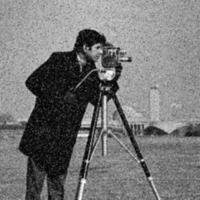
\includegraphics[width=16mm]{Figures/results_mean/cameraman_sp_f.jpg}}\\
        \subfigure{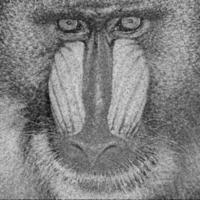
\includegraphics[width=16mm]{Figures/results_mean/baboon_sp_f.jpg}}
      \end{varwidth}
      \begin{varwidth}{0.5\linewidth}
        \subfigure{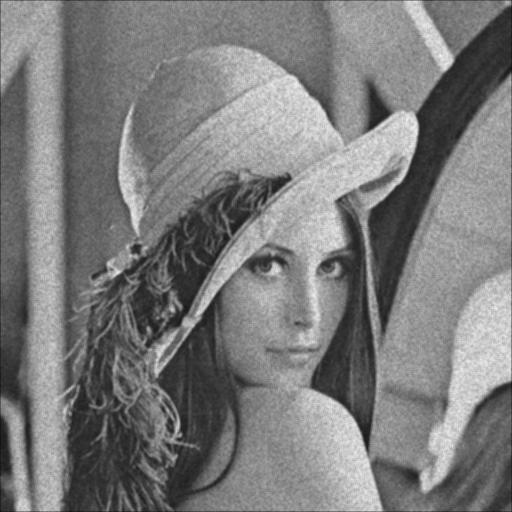
\includegraphics[width=16mm]{Figures/results_mean/lena_spec.jpg}}\\
        \subfigure{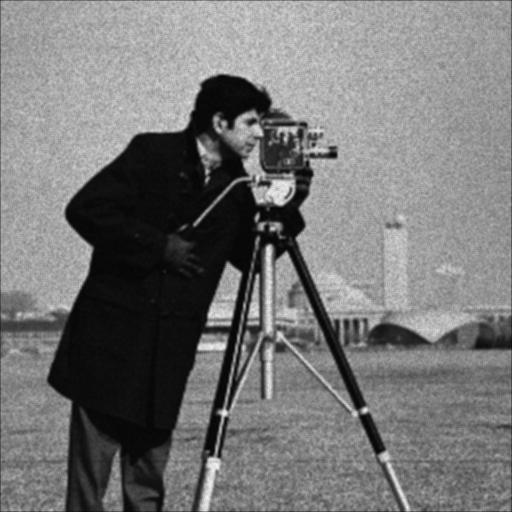
\includegraphics[width=16mm]{Figures/results_mean/cameraman_spec.jpg}}\\
        \subfigure{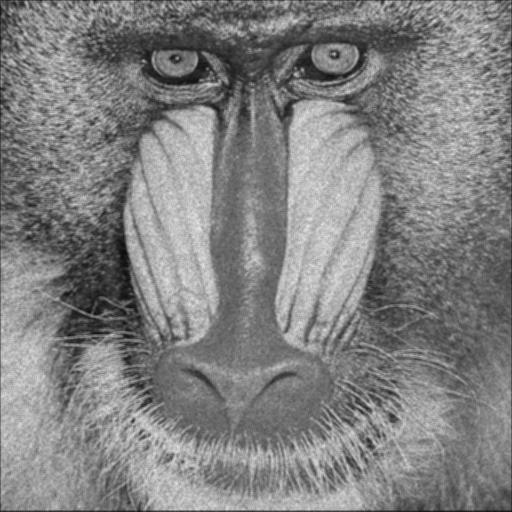
\includegraphics[width=16mm]{Figures/results_mean/baboon_spec.jpg}}
      \end{varwidth}
  	\end{tabular}
  \caption{Denoised images with the mean filter. From left to right: removing Gaussian, Rician, uniform, salt and pepper and speckle noise, respectively.} 
  \label{fig:results_synthetic_mean}
\end{figure}



\subsubsection{Median filter}
	This specialized technique is about as simple as mean filtering, but offers far superior results in special cases. The median filter is particularly well suited for noise which varies greatly from image values, such as salt-and-pepper noise. As we can see in the results, the median filter outperformed every other method when applied to pure salt-and-pepper noise, because evaluating the median always removes outlying values. Unfortunately, median filtering is much less effective on other forms of noise which are more similar to most real-world noise sources. Except for its outstanding results on salt-and-pepper noise, the median filter is inferior to most other techniques on all of the test images.

\begin{figure}[H]
  \centering
  \begin{tabular}{c c c c c}
      \begin{varwidth}{0.5\linewidth}
        \subfigure{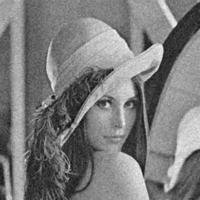
\includegraphics[width=16mm]{Figures/results_median/lena_nor_f.jpg}}\\
        \subfigure{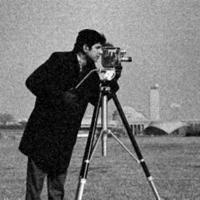
\includegraphics[width=16mm]{Figures/results_median/cameraman_nor_f.jpg}}\\
        \subfigure{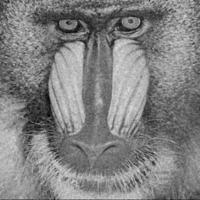
\includegraphics[width=16mm]{Figures/results_median/baboon_nor_f.jpg}}
      \end{varwidth}
      \begin{varwidth}{0.5\linewidth}
        \subfigure{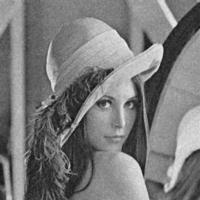
\includegraphics[width=16mm]{Figures/results_median/lena_ric_f.jpg}}\\
        \subfigure{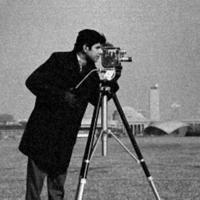
\includegraphics[width=16mm]{Figures/results_median/cameraman_ric_f.jpg}}\\
        \subfigure{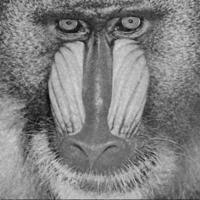
\includegraphics[width=16mm]{Figures/results_median/baboon_ric_f.jpg}}
      \end{varwidth}
      \begin{varwidth}{0.5\linewidth}
        \subfigure{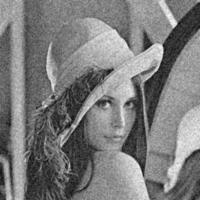
\includegraphics[width=16mm]{Figures/results_median/lena_uni_f.jpg}}\\
        \subfigure{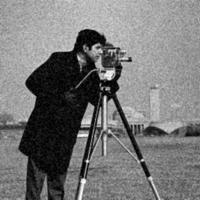
\includegraphics[width=16mm]{Figures/results_median/cameraman_uni_f.jpg}}\\
        \subfigure{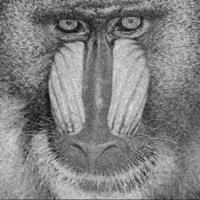
\includegraphics[width=16mm]{Figures/results_median/baboon_uni_f.jpg}}
      \end{varwidth}
      \begin{varwidth}{0.5\linewidth}
        \subfigure{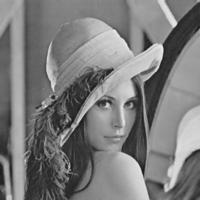
\includegraphics[width=16mm]{Figures/results_median/lena_sp_f.jpg}}\\
        \subfigure{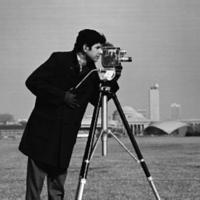
\includegraphics[width=16mm]{Figures/results_median/cameraman_sp_f.jpg}}\\
        \subfigure{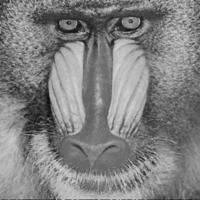
\includegraphics[width=16mm]{Figures/results_median/baboon_sp_f.jpg}}
      \end{varwidth}
      \begin{varwidth}{0.5\linewidth}
        \subfigure{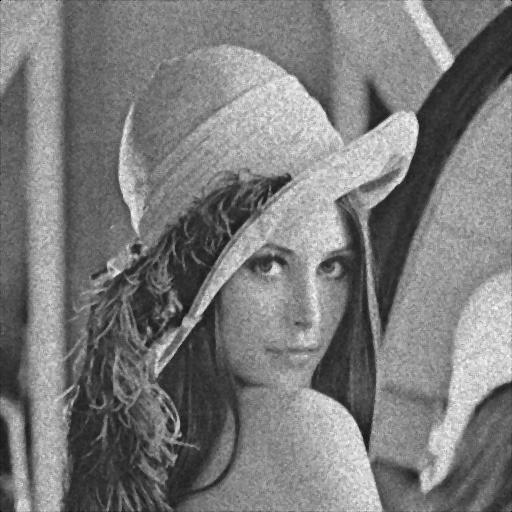
\includegraphics[width=16mm]{Figures/results_median/lena_spec.jpg}}\\
        \subfigure{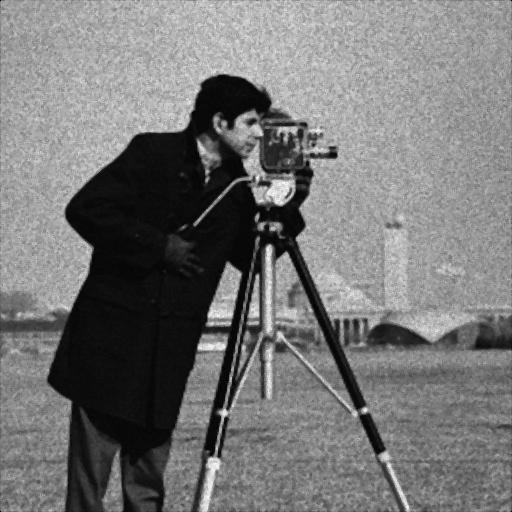
\includegraphics[width=16mm]{Figures/results_median/cameraman_spec.jpg}}\\
        \subfigure{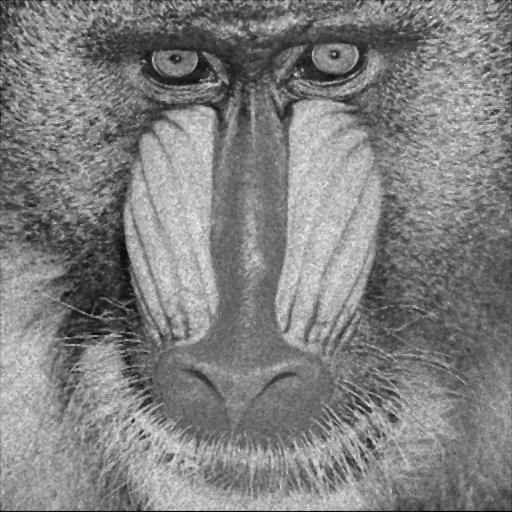
\includegraphics[width=16mm]{Figures/results_median/baboon_spec.jpg}}
      \end{varwidth}
  	\end{tabular}
  \caption{Denoised images with the median filter. From left to right: removing Gaussian, Rician, uniform, salt and pepper and speckle noise, respectively.} 
  \label{fig:results_synthetic_median}
\end{figure}



\subsubsection{LS filter}
When we compare the performance of LS filter with other filters, the results actually are not good at all. it turns out that all the PSNR of denoised output are worse than other advanced methods (expect the other 3 basic filters). This is reasonable because LS filter is at least 25 years older than all advanced methods and technology developed faster year by year. 

However, even when we put the results from LS filter and results from other basic filters in the same table, it is still a little disappointing. Expect for wavelet filter which is the worst, LS filter does not outperform mean and median filter. Only for uniform noise, LS filter do a bit better job than median, but still worse than mean filter.

When we consider the reason why this filter cannot perform very well, we find out that, in the flat area, the method can perform as well as mean filter. But edge preservation is a very important characteristics of LS, which is better than other basic filters. And out of the same reason, it would keep the noise around edges as well. That's probably why it is not better than mean filter in denoising area.  

\begin{figure}[H]
  \centering
  \begin{tabular}{c c c c c}
      \begin{varwidth}{0.5\linewidth}
        \subfigure{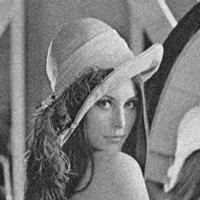
\includegraphics[width=16mm]{Figures/results_Lee/lena_nor-denoised.jpg}}\\
        \subfigure{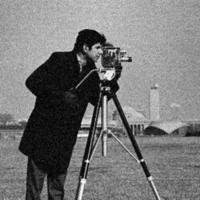
\includegraphics[width=16mm]{Figures/results_Lee/cameraman_nor-denoised.jpg}}\\
        \subfigure{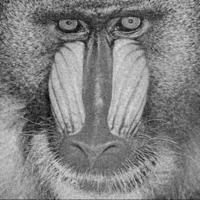
\includegraphics[width=16mm]{Figures/results_Lee/baboon_nor-denoised.jpg}}
      \end{varwidth}
      \begin{varwidth}{0.5\linewidth}
        \subfigure{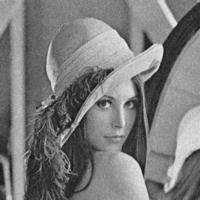
\includegraphics[width=16mm]{Figures/results_Lee/lena_ric-denoised.jpg}}\\
        \subfigure{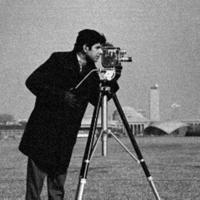
\includegraphics[width=16mm]{Figures/results_Lee/cameraman_ric-denoised.jpg}}\\
        \subfigure{\includegraphics[width=16mm]{Figures/results_Lee/baboon_ric-denoised.jpg}}
      \end{varwidth}
      \begin{varwidth}{0.5\linewidth}
        \subfigure{\includegraphics[width=16mm]{Figures/results_Lee/lena_uni-denoised.jpg}}\\
        \subfigure{\includegraphics[width=16mm]{Figures/results_Lee/cameraman_uni-denoised.jpg}}\\
        \subfigure{\includegraphics[width=16mm]{Figures/results_Lee/baboon_uni-denoised.jpg}}
      \end{varwidth}
      \begin{varwidth}{0.5\linewidth}
        \subfigure{\includegraphics[width=16mm]{Figures/results_Lee/lena_sp-denoised.jpg}}\\
        \subfigure{\includegraphics[width=16mm]{Figures/results_Lee/cameraman_sp-denoised.jpg}}\\
        \subfigure{\includegraphics[width=16mm]{Figures/results_Lee/baboon_sp-denoised.jpg}}
      \end{varwidth}
      \begin{varwidth}{0.5\linewidth}
        \subfigure{\includegraphics[width=16mm]{Figures/results_Lee/lena_spec.jpg}}\\
        \subfigure{\includegraphics[width=16mm]{Figures/results_Lee/cameraman_spec.jpg}}\\
        \subfigure{\includegraphics[width=16mm]{Figures/results_Lee/baboon_spec.jpg}}
      \end{varwidth}
  	\end{tabular}
  \caption{Denoised images with the LS filter. From left to right: removing Gaussian, Rician, uniform, salt and pepper and speckle noise, respectively.} 
  \label{fig:results_synthetic_ls}
\end{figure}

\subsubsection{Wavelet filter}
Fig.\ref{fig:results_synthetic_wavelet} shows the results of the proposed images after the median filter is applied. As observed from the results represented in Section \ref{sc:final-remarks}, the Wavelet filter does not perform better than other methods.

\begin{figure}[H]
  \centering
  \begin{tabular}{c c c c c}
      \begin{varwidth}{0.5\linewidth}
        \subfigure{\includegraphics[width=16mm]{Figures/results_wavelet/lena_nor.jpg}}\\
        \subfigure{\includegraphics[width=16mm]{Figures/results_wavelet/cameraman_nor.jpg}}\\
        \subfigure{\includegraphics[width=16mm]{Figures/results_wavelet/baboon_nor.jpg}}
      \end{varwidth}
      \begin{varwidth}{0.5\linewidth}
        \subfigure{\includegraphics[width=16mm]{Figures/results_wavelet/lena_ric.jpg}}\\
        \subfigure{\includegraphics[width=16mm]{Figures/results_wavelet/cameraman_ric.jpg}}\\
        \subfigure{\includegraphics[width=16mm]{Figures/results_wavelet/baboon_ric.jpg}}
      \end{varwidth}
      \begin{varwidth}{0.5\linewidth}
        \subfigure{\includegraphics[width=16mm]{Figures/results_wavelet/lena_uni.jpg}}\\
        \subfigure{\includegraphics[width=16mm]{Figures/results_wavelet/cameraman_uni.jpg}}\\
        \subfigure{\includegraphics[width=16mm]{Figures/results_wavelet/baboon_uni.jpg}}
      \end{varwidth}
      \begin{varwidth}{0.5\linewidth}
        \subfigure{\includegraphics[width=16mm]{Figures/results_wavelet/lena_sp.jpg}}\\
        \subfigure{\includegraphics[width=16mm]{Figures/results_wavelet/cameraman_sp.jpg}}\\
        \subfigure{\includegraphics[width=16mm]{Figures/results_wavelet/baboon_sp.jpg}}
      \end{varwidth}
      \begin{varwidth}{0.5\linewidth}
        \subfigure{\includegraphics[width=16mm]{Figures/results_wavelet/lena_spec.jpg}}\\
        \subfigure{\includegraphics[width=16mm]{Figures/results_wavelet/cameraman_spec.jpg}}\\
        \subfigure{\includegraphics[width=16mm]{Figures/results_wavelet/baboon_spec.jpg}}
      \end{varwidth}
  	\end{tabular}
  \caption{Denoised images with the wavelet filter. From left to right: removing Gaussian, Rician, uniform, salt and pepper and speckle noise, respectively.} 
  \label{fig:results_synthetic_wavelet}
\end{figure}


\subsubsection{Subspace filter}
Fig.\ref{fig:results_synthetic_subspace} shows the results of the proposed images after the subspace filter is applied.
\begin{figure}[H]
  \centering
  \begin{tabular}{c c c c c}
      \begin{varwidth}{0.5\linewidth}
        \subfigure{\includegraphics[width=16mm]{Figures/results_subspace/lena_nor.jpg}}\\
        \subfigure{\includegraphics[width=16mm]{Figures/results_subspace/cameraman_nor.jpg}}\\
        \subfigure{\includegraphics[width=16mm]{Figures/results_subspace/baboon_nor.jpg}}
      \end{varwidth}
      \begin{varwidth}{0.5\linewidth}
        \subfigure{\includegraphics[width=16mm]{Figures/results_subspace/lena_ric.jpg}}\\
        \subfigure{\includegraphics[width=16mm]{Figures/results_subspace/cameraman_ric.jpg}}\\
        \subfigure{\includegraphics[width=16mm]{Figures/results_subspace/baboon_ric.jpg}}
      \end{varwidth}
      \begin{varwidth}{0.5\linewidth}
        \subfigure{\includegraphics[width=16mm]{Figures/results_subspace/lena_uni.jpg}}\\
        \subfigure{\includegraphics[width=16mm]{Figures/results_subspace/cameraman_uni.jpg}}\\
        \subfigure{\includegraphics[width=16mm]{Figures/results_subspace/baboon_uni.jpg}}
      \end{varwidth}
      \begin{varwidth}{0.5\linewidth}
        \subfigure{\includegraphics[width=16mm]{Figures/results_subspace/lena_sp.jpg}}\\
        \subfigure{\includegraphics[width=16mm]{Figures/results_subspace/cameraman_sp.jpg}}\\
        \subfigure{\includegraphics[width=16mm]{Figures/results_subspace/baboon_sp.jpg}}
      \end{varwidth}
      \begin{varwidth}{0.5\linewidth}
        \subfigure{\includegraphics[width=16mm]{Figures/results_subspace/lena_spec.jpg}}\\
        \subfigure{\includegraphics[width=16mm]{Figures/results_subspace/cameraman_spec.jpg}}\\
        \subfigure{\includegraphics[width=16mm]{Figures/results_subspace/baboon_spec.jpg}}
      \end{varwidth}
  	\end{tabular}
  \caption{Denoised images with the subspace filter. From left to right: removing Gaussian, Rician, uniform, salt and pepper and speckle noise, respectively.} 
  \label{fig:results_synthetic_subspace}
\end{figure}

\begin{figure}[H]
  \centering
      \subfigure{\includegraphics[width=80mm]{Figures/results_subspace/_comparison.jpg}}
  \caption{Graphical comparison of the subspace filter with traditional filtering techniques.} 
  \label{fig:results_synthetic_subspace_evaluation}
\end{figure}


\subsubsection{BMxD filter}
Fig.\ref{fig:results_synthetic_bmxd} shows the results of the proposed images after the BMxD filter is applied.
\begin{figure}[H]
  \centering
  \begin{tabular}{c c c c c}
      \begin{varwidth}{0.5\linewidth}
        \subfigure{\includegraphics[width=16mm]{Figures/results_BMxD/Denoisylena_nor.jpg}}\\
        \subfigure{\includegraphics[width=16mm]{Figures/results_BMxD/Denoisycameraman_nor.jpg}}\\
        \subfigure{\includegraphics[width=16mm]{Figures/results_BMxD/Denoisybaboon_nor.jpg}}
      \end{varwidth}
      \begin{varwidth}{0.5\linewidth}
        \subfigure{\includegraphics[width=16mm]{Figures/results_BMxD/Denoisylena_ric.jpg}}\\
        \subfigure{\includegraphics[width=16mm]{Figures/results_BMxD/Denoisycameraman_ric.jpg}}\\
        \subfigure{\includegraphics[width=16mm]{Figures/results_BMxD/Denoisybaboon_ric.jpg}}
      \end{varwidth}
      \begin{varwidth}{0.5\linewidth}
        \subfigure{\includegraphics[width=16mm]{Figures/results_BMxD/Denoisylena_uni.jpg}}\\
        \subfigure{\includegraphics[width=16mm]{Figures/results_BMxD/Denoisycameraman_uni.jpg}}\\
        \subfigure{\includegraphics[width=16mm]{Figures/results_BMxD/Denoisybaboon_uni.jpg}}
      \end{varwidth}
      \begin{varwidth}{0.5\linewidth}
        \subfigure{\includegraphics[width=16mm]{Figures/results_BMxD/Denoisylena_sp.jpg}}\\
        \subfigure{\includegraphics[width=16mm]{Figures/results_BMxD/Denoisycameraman_sp.jpg}}\\
        \subfigure{\includegraphics[width=16mm]{Figures/results_BMxD/Denoisybaboon_sp.jpg}}
      \end{varwidth}
      \begin{varwidth}{0.5\linewidth}
        \subfigure{\includegraphics[width=16mm]{Figures/results_BMxD/Denoisylena_spec.jpg}}\\
        \subfigure{\includegraphics[width=16mm]{Figures/results_BMxD/Denoisycameraman_spec.jpg}}\\
        \subfigure{\includegraphics[width=16mm]{Figures/results_BMxD/Denoisybaboon_spec.jpg}}
      \end{varwidth}
  	\end{tabular}
  \caption{Denoised images with the BMxD filter. From left to right: removing Gaussian, Rician, uniform, salt and pepper and speckle noise, respectively.} 
  \label{fig:results_synthetic_bmxd}
\end{figure}

\begin{figure}[H]
  \centering
      \subfigure{\includegraphics[width=80mm]{Figures/results_BMxD/_comparison.jpg}}
  \caption{Comparison of the BMxD filter with traditional filtering techniques.} 
  \label{fig:results_synthetic_bmxd_evaluation}
\end{figure}

The denoised images appear sharp and well reconstructed after passing through BM3D algorithm. Only salt and pepper noised images look a bit pixelate.

Values of PSNR are quite important for Gaussian, Rician and Uniform noise. The results exceed those from Mean, Median and Wavelet methods on all the synthetic images. The BM3D method get nevertheless worth PSNR than Median filter on the Salt and Pepper noise, which is a known technique for this type of noise.

Results of PSNR on "baboon" noised images  appear less high than on "Lena" and "cameraman", because there is no big uniform regions and no repetitive pattern in this one, which are regions where this algorithm performs good results. 

\subsubsection{K-SVD filter}
Fig. \ref{fig:results_synthetic_ksvd} shows the results of the proposed images after K-SVD filter is applied. As observed from the colormap set and the results represented in Section \ref{sc:final-remarks}, the filter has a better performance on Gaussian, uniform and speckle noise. However, its performance is not remarkable when denoising high-frequency images.

\begin{figure}[H]
  \centering
  \begin{tabular}{c c c c c}
      \begin{varwidth}{0.5\linewidth}
        \subfigure{\includegraphics[width=16mm]{Figures/results_KSVD/lena_nor.jpg}}\\
        \subfigure{\includegraphics[width=16mm]{Figures/results_KSVD/cameraman_nor.jpg}}\\
        \subfigure{\includegraphics[width=16mm]{Figures/results_KSVD/baboon_nor.jpg}}
      \end{varwidth}
      \begin{varwidth}{0.5\linewidth}
        \subfigure{\includegraphics[width=16mm]{Figures/results_KSVD/lena_ric.jpg}}\\
        \subfigure{\includegraphics[width=16mm]{Figures/results_KSVD/cameraman_ric.jpg}}\\
        \subfigure{\includegraphics[width=16mm]{Figures/results_KSVD/baboon_ric.jpg}}
      \end{varwidth}
      \begin{varwidth}{0.5\linewidth}
        \subfigure{\includegraphics[width=16mm]{Figures/results_KSVD/lena_uni.jpg}}\\
        \subfigure{\includegraphics[width=16mm]{Figures/results_KSVD/cameraman_uni.jpg}}\\
        \subfigure{\includegraphics[width=16mm]{Figures/results_KSVD/baboon_uni.jpg}}
      \end{varwidth}
      \begin{varwidth}{0.5\linewidth}
        \subfigure{\includegraphics[width=16mm]{Figures/results_KSVD/lena_sp.jpg}}\\
        \subfigure{\includegraphics[width=16mm]{Figures/results_KSVD/cameraman_sp.jpg}}\\
        \subfigure{\includegraphics[width=16mm]{Figures/results_KSVD/baboon_sp.jpg}}
      \end{varwidth}
      \begin{varwidth}{0.5\linewidth}
        \subfigure{\includegraphics[width=16mm]{Figures/results_KSVD/lena_spec.jpg}}\\
        \subfigure{\includegraphics[width=16mm]{Figures/results_KSVD/cameraman_spec.jpg}}\\
        \subfigure{\includegraphics[width=16mm]{Figures/results_KSVD/baboon_spec.jpg}}
      \end{varwidth}
  	\end{tabular}
  \caption{Denoised images with the K-SVD filter. From left to right: removing Gaussian, Rician, uniform, salt and pepper and speckle noise, respectively.} 
  \label{fig:results_synthetic_ksvd}
\end{figure}

The comparative results are shown in Fig. \ref{fig:results_synthetic_ksvd_evaluation}. It can be seen that the PSNR of the initial noise is improved in most of the cases except for Baboon test set in which the results are the same or worse. In general, Baboon is the test set leading to the worst restoration for all the evaluated algorithms. This fact could be a consequence of the characteristics of the spiky hair of the baboon. These spikes form a set of edges which can be ``easily'' affected by adding noise and also by restoring with the considered algorithms. Thus, when the denoising process is carried out on this section, most of it, which is formed by high frequencies, is lost.

\begin{figure}[H]
  \centering
      \subfigure{\includegraphics[width=80mm]{Figures/results_KSVD/_comparison.jpg}}
  \caption{Comparison of the K-SVD filter with traditional filtering techniques.} 
  \label{fig:results_synthetic_ksvd_evaluation}
\end{figure}

K-SVD algorithm is able to remove noise from the different test images. However, its performance was not always the best. It can be observed that in some cases, the values of PSNR for mean filter and median filter are higher than the ones for K-SVD. Contrarily, we see that the wavelet filter does not succeed in filtering any of the types of noise, compared to other methods. 

As expected, median filter outperforms when evaluated under salt and pepper noise in comparison with the other algorithms. 


\subsubsection{NLM filter}
Fig.\ref{fig:results_synthetic_nlm} shows the results of the proposed images after the NLM filter is applied.
\begin{figure}[H]
  \centering
  \begin{tabular}{c c c c c}
      \begin{varwidth}{0.5\linewidth}
        \subfigure{\includegraphics[width=16mm]{Figures/results_NLM/Lena_g_den.jpg}}\\
        \subfigure{\includegraphics[width=16mm]{Figures/results_NLM/Cameraman_g_den.jpg}}\\
        \subfigure{\includegraphics[width=16mm]{Figures/results_NLM/Baboon_g_den.jpg}}
      \end{varwidth}
      \begin{varwidth}{0.5\linewidth}
        \subfigure{\includegraphics[width=16mm]{Figures/results_NLM/Lena_rc_den.jpg}}\\
        \subfigure{\includegraphics[width=16mm]{Figures/results_NLM/Cameraman_rc_den.jpg}}\\
        \subfigure{\includegraphics[width=16mm]{Figures/results_NLM/Baboon_rc_den.jpg}}
      \end{varwidth}
      \begin{varwidth}{0.5\linewidth}
        \subfigure{\includegraphics[width=16mm]{Figures/results_NLM/Lena_u_den.jpg}}\\
        \subfigure{\includegraphics[width=16mm]{Figures/results_NLM/Cameraman_u_den.jpg}}\\
        \subfigure{\includegraphics[width=16mm]{Figures/results_NLM/Baboon_u_den.jpg}}
      \end{varwidth}
      \begin{varwidth}{0.5\linewidth}
        \subfigure{\includegraphics[width=16mm]{Figures/results_NLM/Lena_snp_den.jpg}}\\
        \subfigure{\includegraphics[width=16mm]{Figures/results_NLM/Cameraman_snp_den.jpg}}\\
        \subfigure{\includegraphics[width=16mm]{Figures/results_NLM/Baboon_snp_den.jpg}}
      \end{varwidth}
      \begin{varwidth}{0.5\linewidth}
        \subfigure{\includegraphics[width=16mm]{Figures/results_NLM/Lena_spec_den.jpg}}\\
        \subfigure{\includegraphics[width=16mm]{Figures/results_NLM/Cameraman_spec_den.jpg}}\\
        \subfigure{\includegraphics[width=16mm]{Figures/results_NLM/Baboon_spec_den.jpg}}
      \end{varwidth}
  	\end{tabular}
  \caption{Denoised images with the NLM and OBNLM filter. From left to right: removing Gaussian, Rician, uniform, and salt and pepper noise with NLM and speckle noise with OBNLM, respectively.} 
  \label{fig:results_synthetic_nlm}
\end{figure}

\begin{figure}[H]
  \centering
      \subfigure{\includegraphics[width=80mm]{Figures/results_NLM/_comparison.jpg}}
  \caption{Comparison of the NLM filter with traditional filtering techniques.} 
  \label{fig:results_synthetic_nlm_evaluation}
\end{figure}

The results for NLM and OBNLM filters are presented in Fig. \ref{fig:results_synthetic_nlm}. The human eye is the best testing mechanism to measure the quality of the restored images. The NLM filters produce good qualitative results except falling second to median filters in case of salt and pepper noise. OBNLM produces similarly good results while denoising images with speckle noise. 

The NLM filters are not associated with any geometrical shapes. In other words there are no geometrical structures in the residual images. This property allows these filters to work irrespective of the nature of the original image. So, the edges will always be retained which is a big advantage of NLM over several other filters.

The best results for NLM are obtained on periodic and textured images as is the case in the image of the baboon. However, in case of cameraman image, one can see the presence of artifacts in the smooth background of the image. This owes greatly to the fact that for every pixel, the algorithm can find a large set of similar pixels in the neighborhood to compute the new value.  


\subsubsection{PGPD filter}
Fig.\ref{fig:results_synthetic_pgpd} shows the results of the proposed images after the PGPD filter is applied.
\begin{figure}[H]
  \centering
  \begin{tabular}{c c c c c}
      \begin{varwidth}{0.5\linewidth}
        \subfigure{\includegraphics[width=16mm]{Figures/results_PGPD/lena_nor_PGPD.jpg}}\\
        \subfigure{\includegraphics[width=16mm]{Figures/results_PGPD/cameraman_nor_PGPD.jpg}}\\
        \subfigure{\includegraphics[width=16mm]{Figures/results_PGPD/baboon_nor_PGPD.jpg}}
      \end{varwidth}
      \begin{varwidth}{0.5\linewidth}
        \subfigure{\includegraphics[width=16mm]{Figures/results_PGPD/lena_ric_PGPD.jpg}}\\
        \subfigure{\includegraphics[width=16mm]{Figures/results_PGPD/cameraman_ric_PGPD.jpg}}\\
        \subfigure{\includegraphics[width=16mm]{Figures/results_PGPD/baboon_ric_PGPD.jpg}}
      \end{varwidth}
      \begin{varwidth}{0.5\linewidth}
        \subfigure{\includegraphics[width=16mm]{Figures/results_PGPD/lena_uni_PGPD.jpg}}\\
        \subfigure{\includegraphics[width=16mm]{Figures/results_PGPD/cameraman_uni_PGPD.jpg}}\\
        \subfigure{\includegraphics[width=16mm]{Figures/results_PGPD/baboon_uni_PGPD.jpg}}
      \end{varwidth}
      \begin{varwidth}{0.5\linewidth}
        \subfigure{\includegraphics[width=16mm]{Figures/results_PGPD/lena_sp_PGPD.jpg}}\\
        \subfigure{\includegraphics[width=16mm]{Figures/results_PGPD/cameraman_sp_PGPD.jpg}}\\
        \subfigure{\includegraphics[width=16mm]{Figures/results_PGPD/baboon_sp_PGPD.jpg}}
      \end{varwidth}
      \begin{varwidth}{0.5\linewidth}
        \subfigure{\includegraphics[width=16mm]{Figures/results_PGPD/lena_spec_PGPD.jpg}}\\
        \subfigure{\includegraphics[width=16mm]{Figures/results_PGPD/cameraman_spec_PGPD.jpg}}\\
        \subfigure{\includegraphics[width=16mm]{Figures/results_PGPD/baboon_spec_PGPD.jpg}}
      \end{varwidth}
  	\end{tabular}
  \caption{Denoised images with the PGPD filter. From left to right: removing Gaussian, Rician, uniform, salt and pepper and speckle noise, respectively.} 
  \label{fig:results_synthetic_pgpd}
\end{figure}

\begin{figure}[H]
  \centering
      \subfigure{\includegraphics[width=80mm]{Figures/results_PGPD/_comparison.jpg}}
  \caption{Comparison of the PGPD filter with traditional filtering techniques.} 
  \label{fig:results_synthetic_pgpd_evaluation}
\end{figure}

The PGPD filter has better performance than the median filter in terms of removing Guassion noise, uniform noise and Rician noise. But in case of salt and pepper noise the median filter is showing better performance than the PGPD.This could happen due to the nature of Salt and Pepper noise itself; Indeed, Salt and Pepper has random distribution  with 100\% error in each pixel it apperars which makes it hard to take into account the noise while grouping patches into a PG, therefore it brings the efficiency of algorithm down dramatically.

When we compare the PGPD filter with mean filter the PGPD filter is better in removing Gaussian noise, uniform noise, and Rician noise. 

In all types of noise we use, the PGPD filter results have better PSNR than the Lee filter.  Lee filter is known for its characteriscs of edge preservation, but according to the Figure \ref{fig:results_synthetic_pgpd_evaluation}, the image filtered by PGPD has better visual accuracy than the images filtered by Lee, so we can draw the conclusion that PGPD filter preserves edges even better. 

PSNR of each denoised image using PGPD is greater than the one denoised by the Hard- and soft-thresholding in wavelet domain.

We can draw a conclusion that PGPD denoising performance provides great PSNR result no matter what the noise is present in the picture, except for Salt and Pepper. When it comes to salt and pepper noise it becomes hard to align patches due to the nature of the noise: salt and pepper give the 100\% error per pixel while matching 2 patches which reduces the efficiency of the algorithm.


%%%	%%%	%%%
\subsection{Retinopathy images} 
In this section the obtained results when denoising retinopathy images are shown and evaluated.
%\subsubsection{Mean filter}
%
%\begin{figure}[H]
%  \centering
%      \subfigure{\includegraphics[width=80mm]{Figures/non2.jpg}}
%  \caption{Denoised retinopathy image with the mean filter.} 
%  \label{fig:results_rimage_mean}
%\end{figure}
%
%\begin{figure}[H]
%  \centering
%      \subfigure{\includegraphics[width=80mm]{Figures/non2.jpg}}
%  \caption{Segmentation of a retinopathy volume after denoising using the mean filter.} 
%  \label{fig:results_rsegmentation_mean}
%\end{figure}
%
%\subsubsection{Median filter}
%
%\begin{figure}[H]
%  \centering
%      \subfigure{\includegraphics[width=80mm]{Figures/non2.jpg}}
%  \caption{Denoised retinopathy image with the median filter.} 
%  \label{fig:results_rimage_median}
%\end{figure}
%
%\begin{figure}[H]
%  \centering
%      \subfigure{\includegraphics[width=80mm]{Figures/non2.jpg}}
%  \caption{Segmentation of a retinopathy volume after denoising using the median filter.} 
%  \label{fig:results_rsegmentation_median}
%\end{figure}
%
%
%\subsubsection{Wavelet filter}
%
%\begin{figure}[H]
%  \centering
%      \subfigure{\includegraphics[width=80mm]{Figures/non2.jpg}}
%  \caption{Denoised retinopathy image with the wavelet filter.} 
%  \label{fig:results_rimage_wavelet}
%\end{figure}
%
%\begin{figure}[H]
%  \centering
%      \subfigure{\includegraphics[width=80mm]{Figures/non2.jpg}}
%  \caption{Segmentation of a retinopathy volume after denoising using the wavelet filter.} 
%  \label{fig:results_rsegmentation_wavelet}
%\end{figure}


\subsubsection{Subspace filter}
-
\begin{figure}[H]
  \centering
      \subfigure{\includegraphics[width=80mm]{Figures/results_subspace/retinopathy_image.jpg}}
  \caption{Denoised retinopathy image with the subspace filter.} 
  \label{fig:results_rimage_subspace}
\end{figure}

\begin{figure}[H]
  \centering
      \subfigure{\includegraphics[width=80mm]{Figures/results_subspace/retinopathy_segmentation.jpg}}
  \caption{Segmentation of a retinopathy volume after denoising using the subspace filter.} 
  \label{fig:results_rsegmentation_subspace}
\end{figure}



\subsubsection{BMxD filter}
Comparing the results of the denoised retinopathy image with other techniques, the method is still one of the most successful. However, there are less gap between the PSNRs obtained from the retinopathy image denoised with this method and the others, than the PSNRs obtained from the denoised synthetic images with the same methods. 

\begin{figure}[H]
  \centering
      \subfigure{\includegraphics[width=80mm]{Figures/results_BMxD/retinopathy_image.jpg}}
  \caption{Denoised retinopathy image with the BMxD filter.} 
  \label{fig:results_rimage_bmxd}
\end{figure}

\begin{figure}[H]
  \centering
      \subfigure{\includegraphics[width=80mm]{Figures/results_BMxD/retinopathy_segmentation.jpg}}
  \caption{Segmentation of a retinopathy volume after denoising using the BMxD filter.} 
  \label{fig:results_rsegmentation_bmxd}
\end{figure}



\subsubsection{KSVD filter}
 In general terms, K-SVD is able to reduce noise on the image without affecting the key components (the layers on the images) more than the other algorithms.
 
\begin{figure}[H]
  \centering
      \subfigure{\includegraphics[width=80mm]{Figures/results_KSVD/retinopathy_image.jpg}}
  \caption{Denoised retinopathy image with the K-SVD filter.} 
  \label{fig:results_rimage_ksvd}
\end{figure}

\begin{figure}[H]
  \centering
      \subfigure{\includegraphics[width=80mm]{Figures/results_KSVD/retinopathy_segmentation.jpg}}
  \caption{Segmentation of a retinopathy volume after denoising using the K-SVD filter.} 
  \label{fig:results_rsegmentation_ksvd}
\end{figure}



\subsubsection{NLM filter}
 We denoised the images using Non-Linear Means (NLM) filter, However, when we segmented the images, the output was not much different in comparison to the segmentation of original noisy images. 
\begin{figure}[H]
  \centering
      \subfigure{\includegraphics[width=80mm]{Figures/results_NLM/retinopathy_image.jpg}}
  \caption{Denoised retinopathy image with the NLM filter.} 
  \label{fig:results_rimage_nlm}
\end{figure}

\begin{figure}[H]
  \centering
      \subfigure{\includegraphics[width=80mm]{Figures/results_NLM/retinopathy_segmentation.jpg}}
  \caption{Segmentation of a retinopathy volume after denoising using the NLM filter.} 
  \label{fig:results_rsegmentation_nlm}
\end{figure}


\subsubsection{PGPD filter}
-
\begin{figure}[H]
  \centering
      \subfigure{\includegraphics[width=80mm]{Figures/results_PGPD/retinopathy_image.jpg}}
  \caption{Denoised retinopathy image with the PGPD filter.} 
  \label{fig:results_rimage_pgpd}
\end{figure}

\begin{figure}[H]
  \centering
      \subfigure{\includegraphics[width=80mm]{Figures/results_PGPD/retinopathy_segmentation.jpg}}
  \caption{Segmentation of a retinopathy volume after denoising using the PGPD filter.} 
  \label{fig:results_rsegmentation_pgpd}
\end{figure}

\subsubsection{SD-OCT Evaluation}
To provide a quantitative comparison of the denoised retinopathy images with the different methods, we computed the PSNR. In this case, it was performed between the input image and the output of each algorithm. It is clear that although this computation does not give the real PSNR, the obtained value is useful to get an idea of the performance of the different algorithms. The results are presented in Table \ref{tab:numerical_results_retinopathy}. In terms of this approach, K-SVD is able to reduce noise on the image without affecting the key components (the layers on the images) more than the other algorithms.

\begin{table}[H]
	\centering
   	\caption{PSNR for denoising algorithms considering retinopathy images}
	\begin{tabular}{|c|c|}
	\hline
	\textbf{Technique} & \textbf{Retinopathy} \\ \hline
	Subspace & $24.47$ \\ \hline
	BMxD & $25.73$ \\ \hline
	K-SVD & $\textbf{26.68}$ \\ \hline
	NLM & $23.57$ \\ \hline
	PGPD & $23.55$ \\ \hline
	\end{tabular}
	\label{tab:numerical_results_retinopathy}
\end{table}

